\documentclass{article}

% Configuración de idioma
\usepackage[spanish]{babel}
\usepackage[utf8]{inputenc}
\usepackage[T1]{fontenc}

% Tamaño de página y márgenes
\usepackage[letterpaper,top=2cm,bottom=2cm,left=3cm,right=3cm,marginparwidth=1.75cm]{geometry}

% Paquetes útiles
\usepackage{amsmath}
\usepackage{booktabs}
\usepackage{graphicx}
\usepackage[colorlinks=true, allcolors=blue]{hyperref}


\title{Notas para tesis de doctorado 25-I}
\author{Erick Felipe Serrato Garcia}

\begin{document}
\maketitle

\section{Efecto Allee}

The Allee effect is a fenómeno in ecologa and biologa of poblaciones that describes a tasa of crecimiento reducida in densidades poblacionales bajas. Este efecto puede clasificarse en dos tipos: efecto Allee fuerte y efecto Allee débil.

\subsection{Efecto Allee Fuerte}

Para una población $N(t)$, el efecto Allee fuerte se modela con una versión modificada de la ecuación logística:

\begin{equation}
\frac{dN}{dt} = rN \left(1 - \frac{N}{K}\right) \left(\frac{N - A}{K - A}\right)
\label{eq:strong_allee}
\end{equation}

\begin{itemize}
\item $r$: Tasa intrínseca de crecimiento.
\item $K$: Capacidad de carga del ambiente.
\item $A$: Umbral de Allee. Si $N < A$, la población decrece.
\end{itemize}

\subsection{Efecto Allee Débil}

En el efecto Allee débil, la población tiene un crecimiento reducido a bajas densidades, pero no necesariamente se extingue si cae por debajo de $A$:

\begin{equation}
\frac{dN}{dt} = rN \left(1 - \frac{N}{K}\right) \left(\frac{N}{A} - 1\right)
\end{equation}

\begin{itemize}
\item $N > A$: La población crece.
\item $N < A$: La población decrece.
\end{itemize}

\subsection{Relación entre efecto Allee fuerte y débil}

Cuando $A$ está cercano a $K$, se puede aproximar:



Esto permite transformar la ecuación del efecto Allee fuerte \eqref{eq:strong_allee} en:

\begin{equation}
rN \left(1 - \frac{N}{K}\right) \left(\frac{N - A}{K - A}\right) \approx rN \left(1 - \frac{N}{K}\right) \left(\frac{N}{A} - 1\right)
\end{equation}

\subsection{Aplicación al modelo tumoral}

\begin{itemize}
\item \textbf{Efecto Allee fuerte:} Aplica si se requiere una cantidad mínima de células cancerígenas para que el tumor crezca. Bajo ese umbral, el tumor no es viable.
\item \textbf{Efecto Allee débil:} Aunque el crecimiento se reduce a baja densidad, el tumor podría persistir bajo el umbral.
\item \textbf{Importancia biológica:} La transición de efecto fuerte a débil puede orientar estrategias terapéuticas que apunten a reducir la densidad celular tumoral a niveles críticos.
\end{itemize}

\section{Modelo}

Definimos las variables: $c$ (células cancerígenas), $s$ (células sanas), $i$ (células inmunes). El modelo dinámico se describe mediante:

\begin{equation}
\frac{dc}{dt} = r_c c \left(\frac{c}{a} - 1\right)\left(1 - \frac{c}{k_c}\right) - \alpha c s - \beta c i - \frac{\mu}{2} (\eta i^2 + \gamma s^2)
\label{eqn:cancer_dynamic}
\end{equation}

\begin{equation}
\frac{ds}{dt} = r_s s \left(1 - \frac{s}{k_s}\right) - \gamma c s + \delta s i^2 - \frac{\mu}{2} \alpha c^2
\label{eqn:sano_dynamic}
\end{equation}

\begin{equation}
\frac{di}{dt} = r_i i \left(1 - \frac{i}{k_i}\right) - \eta c i + \delta s^2 i - \frac{\mu}{2} \beta c^2
\label{eqn:inmune_dynamic}
\end{equation}

\subsection*{Parámetros del modelo}

\begin{table}[H]
\centering
\begin{tabular}{lll}
\toprule
\textbf{Parámetro} & \textbf{Valor} & \textbf{Descripción} \
\midrule
$r_c$ & 5.84 & Tasa de crecimiento de células cancerígenas \
$r_s$ & 13.12 & Tasa de crecimiento de células sanas \
$r_i$ & 10.92 & Tasa de crecimiento de células inmunes \
$k_c$, $k_s$, $k_i$ & 1.00 & Capacidades de carga de cada población \
$a$ & 7.22 & Umbral de crecimiento para células cancerígenas \
$\alpha$ & 10.22 & Inhibición de células sanas por células cancerígenas \
$\beta$ & 7.60 & Inhibición de células inmunes por células cancerígenas \
$\gamma$ & 0.74 & Interacción entre células sanas e inmunes \
$\delta$ & 5.40 & Cooperación entre células sanas e inmunes \
$\eta$ & 5.08 & Eficiencia inmune contra células cancerígenas \
$\mu$ & $\in {0, 1}$ & Activación binaria de la respuesta inmune \
$D_c = D_s = D_i$ & 1.00 & Coeficientes de difusión espacial \
\bottomrule
\end{tabular}
\caption{Valores de los parámetros utilizados en el modelo.}
\end{table}

\section{Resultados: Efecto Allee débil}

\subsection{Estados estacionarios}

Los estados estacionarios se definen como aquellos donde las derivadas temporales se anulan: $\frac{dc}{dt} = \frac{ds}{dt} = \frac{di}{dt} = 0$. Estos puntos representan condiciones de equilibrio entre las tres poblaciones celulares.

\begin{itemize}
\item \textbf{Estable:} El sistema regresa a este punto ante pequeñas perturbaciones. Representa control del tumor.
\item \textbf{Inestable:} Perturbaciones pequeñas pueden llevar al sistema a una proliferación tumoral o colapso inmunológico.
\end{itemize}

\begin{figure}[htbp]
\centering
\includegraphics[width=0.45\textwidth]{images/steady.png}
\includegraphics[width=0.45\textwidth]{images/steady_mu0.png}
\caption{Estados estacionarios obtenidos para $\mu = 1$ (izquierda) y $\mu = 0$ (derecha). Para $\mu = 1$ se observa un punto inestable $P_1(c,s,i) = (1.0826, 0.4885, 0.1649)$ y uno estable $P_2(c,s,i) = (1.7045, 0.3876, -1.2883)$. Para $\mu = 0$ se observa un punto inestable $P_1(c,s,i) = (1.4103, 1.0414, 0.6110)$ y uno estable $P_2(c,s,i) = (2.9271, 1.6416, -1.6532)$.}
\label{fig:steady_gral}
\end{figure}
\subsection{Análisis de estabilidad lineal.}


El análisis de estabilidad lineal para un sistema que modela la interacción entre células cancerosas, células sanas y el sistema inmune nos proporciona información clave sobre cómo pequeñas perturbaciones afectan el comportamiento del sistema en torno a sus estados estacionarios.

El sistema de ecuaciones en nuestro caso es:

\begin{equation}
    \frac{dc}{dt} = D_c \nabla^2 c + r_c c \left(\frac{c}{a} - 1\right)\left(1-\frac{c}{k_c}\right) - \alpha c s^2  - \beta c i^2  - \mu ( \gamma s^2+ \eta i^2),
     \label{eqn:cancer_dynamic_spatial}
\end{equation}

\begin{equation}
    \frac{ds}{dt} = D_s \nabla^2 s + r_s s \left(1 - \frac{s}{k_s}\right) - \gamma s c^2 + \delta s i^2 - \frac{\mu}{2} \alpha s c^2 ,
    \label{eqn:sano_dynamic_spatial}
\end{equation}

\begin{equation}
    \frac{di}{dt} = D_i \nabla^2 i + r_i i \left(1-\frac{i}{k_i}\right) - \eta c^2 i + \delta s^2 i - \frac{\mu}{2}\beta i c^2 .
    \label{eqn:inmune_dynamic_spatial}
\end{equation}


\textbf{Estados estacionarios}
\vspace{0.2cm}


\textbf{Perturbaciones alrededor de los estados estacionarios}
\vspace{0.2cm}

Una vez obtenido el estado estacionario $(c_0, s_0, i_0)$, introducimos pequeñas perturbaciones $\tilde{c}$, $\tilde{s}$ e $\tilde{i}$ alrededor de dicho punto:

\[
c = c_0 + \tilde{c}, \quad s = s_0 + \tilde{s}, \quad i = i_0 + \tilde{i}.
\]

Sustituyendo estas expresiones en las ecuaciones originales, linealizamos el sistema descartando términos de orden superior, es decir, los que contienen productos de perturbaciones como $\tilde{c}^2$, $\tilde{s}^2$, $\tilde{i}^2$, etc.
\vspace{0.5cm}

\textbf{Linealización del sistema}
\vspace{0.2cm}

Al realizar la sustitución, obtenemos un sistema de ecuaciones lineales para las perturbaciones. Este sistema se puede escribir de manera compacta en forma matricial:

\[
\frac{d}{dt} 
\begin{pmatrix}
\tilde{c} \\
\tilde{s} \\
\tilde{i}
\end{pmatrix}
= 
\mathbf{J}
\begin{pmatrix}
\tilde{c} \\
\tilde{s} \\
\tilde{i}
\end{pmatrix}
\]

donde $\mathbf{J}$ es la matriz Jacobiana del sistema, que contiene las derivadas parciales de las ecuaciones con respecto a cada variable evaluadas en el estado estacionario $(c_0, s_0, i_0)$.

\[
\mathbf{J} = 
\begin{pmatrix}
\frac{\partial f_c}{\partial c} & \frac{\partial f_c}{\partial s} & \frac{\partial f_c}{\partial i} \\
\frac{\partial f_s}{\partial c} & \frac{\partial f_s}{\partial s} & \frac{\partial f_s}{\partial i} \\
\frac{\partial f_i}{\partial c} & \frac{\partial f_i}{\partial s} & \frac{\partial f_i}{\partial i}
\end{pmatrix}.
\]

En este caso, las funciones $f_c$, $f_s$ y $f_i$ representan el lado derecho de las ecuaciones dinámicas para las células cancerígenas, sanas y el sistema inmune, respectivamente.
\vspace{0.5cm}

\textbf{Análisis de los autovalores}
\vspace{0.2cm}

Para determinar la estabilidad del sistema, se calculan los autovalores de la matriz Jacobiana $\mathbf{J}$. La estabilidad depende de los valores reales de estos autovalores. Existen tres casos a considerar:

\begin{itemize}
    \item \textbf{Valores reales positivos ($\Re(\lambda) > 0$):} Estos indican una inestabilidad. Si un autovalor tiene una parte real positiva, significa que pequeñas perturbaciones en torno al estado estacionario crecerán exponencialmente en el tiempo, alejando al sistema de ese equilibrio. Esto podría representar un comportamiento descontrolado en el sistema biológico, como el crecimiento rápido de las células cancerosas cuando las condiciones son favorables para ellas.
    
    \item \textbf{Valores reales negativos ($\Re(\lambda) < 0$):} Indican estabilidad. Las perturbaciones se amortiguan, lo que significa que el sistema tenderá a regresar al estado estacionario tras sufrir una pequeña alteración. Esto podría corresponder a un estado donde el sistema inmune logra controlar la proliferación del cáncer.
    
    \item \textbf{Partes imaginarias ($\Im(\lambda)$):} La presencia de partes imaginarias sugiere que las perturbaciones pueden provocar oscilaciones en el sistema. Estas oscilaciones podrían ser indicativas de ciclos periódicos, donde las poblaciones de células sanas, cancerosas y del sistema inmune fluctúan en el tiempo. En un contexto biológico, estas oscilaciones podrían interpretarse como fases de remisión y recurrencia del cáncer, o variaciones cíclicas en la respuesta inmune.
\end{itemize}

Haciendo  un análisis de estabilidad lineal sobre las ecuaciones \ref{eqn:cancer_dynamic}, \ref{eqn:sano_dynamic} y  \ref{eqn:inmune_dynamic}, de la Figura \ref{fig:imagen_estabilidad} podemos discutir lo siguiente:


\begin{itemize}
    \item \textbf{Para $q \approx 0$}, se observa que $\Re(\lambda_3)$ es bastante alto, lo que sugiere que para perturbaciones de baja frecuencia (o de gran longitud de onda), el sistema es inestable. Esto puede indicar una tendencia a la formación de estructuras o patrones grandes, o el desarrollo de un comportamiento no homogéneo en la mezcla de células.
    
    \item \textbf{A medida que \(q\) aumenta} (es decir, para perturbaciones de alta frecuencia o pequeñas longitudes de onda), la parte real de \(\lambda_3\) disminuye y eventualmente se vuelve negativa. Esto indica que el sistema es más estable frente a perturbaciones de menor longitud de onda.
    
\end{itemize}

\begin{figure}[htbp]
    \centering
    \begin{minipage}[b]{0.45\textwidth}
        \centering
        \includegraphics[width=\textwidth]{images/linear_stability_p1.png}
        \caption{Analisis de estabilidad para el estado estacionario $P_1(c,s,i) =  (1.229,1.093,0.045)$}
        \label{fig:imagen1}
    \end{minipage}
    \hfill
    \begin{minipage}[b]{0.45\textwidth}
        \centering
        \includegraphics[width=\textwidth]{images/linear_stability_p2.png}
        \caption{Analisis de estabilidad para el estado estacionario $P_2(c,s,i) = (4.69, 2.15, -2.71)$}
        \label{fig:imagen2}
    \end{minipage}
    \caption{Analisis de estabilidad para los dos estados estacionarios inestables}
    \label{fig:imagen_estabilidad}
\end{figure}


\subsection{Solución numérica}

Implementamos la solución numérica de las ecuaciones diferenciales parciales acopladas que describen la interacción entre las células cancerígenas, células sanas y el sistema inmune, utilizando FEniCS. 

Para las simulaciones, consideramos una evolución temporal de los campos utilizando las siguientes condiciones iniciales aleatorias en los intervalos:

\[
0.2 < c < 0.4, \quad 0.7 < s < 0.9, \quad 0.5 < i < 0.7
\]

Las configuraciones de la simulación son las siguientes:

\begin{itemize}
    \item Tiempo final: $T = 0.215$
    \item Tamaño del paso temporal: $dt = 0.001$
    \item Número de nodos en la discretización espacial: $100$
\end{itemize}

Resolvimos las ecuaciones \ref{eqn:cancer_dynamic_spatial}, \ref{eqn:sano_dynamic_spatial} y \ref{eqn:inmune_dynamic_spatial}, donde las soluciones son calculadas a través de métodos de elementos finitos. El dominio fue discretizado utilizando un mallado uniforme de $100$ nodos y el paso temporal fue establecido en $dt = 0.001$, permitiendo simular la evolución temporal de los campos hasta el tiempo final $T = 0.23$.

Las condiciones iniciales aleatorias fueron generadas para cada campo, asegurando que los valores de $c$, $s$ e $i$ se encontraran dentro de los rangos especificados. Los resultados numéricos obtenidos proporcionan información detallada sobre la evolución y el comportamiento de las dinámicas de interacción entre las células, tanto en términos de estabilidad como de posibles transiciones entre estados.



\begin{figure}[htbp]
    \centering
    \includegraphics[width=1\textwidth, height=0.2\textheight]{images/fields.png}
    \caption{Evolución de los campos inicialmente aleatorio con $0.2< c < 0.4$, $0.7 < s < 0.9$ e $0.5 < i < 0.7$}
    \label{fig:fields_evolution}
\end{figure}



En el siguiente \href{https://drive.google.com/file/d/1lAHa3TRPTFROOFaI3XvsIvU65_pN7HG5/view?usp=sharing}{video}, podemos ver la evolución en el tiempo de nuestro sistema que mostramos en la figua \ref{fig:fields_evolution}. A partir de los resultados numéricos observados en la imagen, que corresponden a los campos del cáncer (c), células sanas (s) y el sistema inmune (i) en el tiempo final de la simulación (T = 0.215), podemos hacer varias observaciones clave sobre las dinámicas y distribuciones espaciales de estas tres poblaciones.

\begin{itemize}
    \item \textbf{Campo del cáncer (c):}
    \begin{itemize}
        \item El campo del cáncer muestra una distribución espacial heterogénea, con regiones localizadas de alta y baja concentración.
        \item Las áreas en rojo representan regiones donde la concentración de células cancerígenas es relativamente alta, mientras que las áreas en azul indican bajas concentraciones.
        \item Esta heterogeneidad espacial sugiere que las células cancerígenas no se distribuyen de manera uniforme, sino que pueden formar agregados o patrones en ciertas zonas. Esto podría indicar inestabilidad espacial o competencia con las células sanas y el sistema inmune.
    \end{itemize}
    
    \item \textbf{Campo de las células sanas (s):}
    \begin{itemize}
        \item El campo de las células sanas presenta un patrón más difuso y de menor contraste en comparación con el cáncer.
        \item Esto podría indicar que la población de células sanas está siendo significativamente afectada o inhibida por la proliferación del cáncer y la acción del sistema inmune.
        \item Las áreas en tonos más oscuros sugieren que las células sanas están en bajas concentraciones en ciertas regiones, lo cual podría ser consecuencia de la invasión cancerígena o de la respuesta inmunitaria en esos sitios.
    \end{itemize}
    
    \item \textbf{Campo del sistema inmune (i):}
    \begin{itemize}
        \item El campo del sistema inmune también muestra una distribución espacial compleja, pero con menos contraste que el cáncer.
        \item Esto podría reflejar que, aunque el sistema inmune está presente en todo el dominio, su activación no es uniforme y es posible que esté concentrado en áreas específicas, donde la presencia del cáncer es más prominente.
        \item Las zonas de mayor intensidad (color amarillo) representan regiones donde el sistema inmune está más activo, posiblemente en respuesta al ataque al cáncer.
    \end{itemize}
\end{itemize}

El comportamiento observado en los tres campos sugiere una interacción compleja entre las tres poblaciones. El hecho de que el campo del cáncer sea más heterogéneo y con áreas de alta concentración podría estar indicando un crecimiento invasivo y agresivo en ciertas zonas, mientras que el campo de las células sanas parece estar más afectado, con una menor presencia en la mayor parte del dominio. Esto sugiere que el cáncer está desplazando a las células sanas. Por otro lado, la presencia del sistema inmune, aunque generalizada, parece estar limitada en su efectividad, ya que no logra eliminar el cáncer por completo en ninguna región específica.
\\

En términos generales, estos resultados sugieren un escenario donde el cáncer está ganando terreno, con una respuesta del sistema inmune que es capaz de reaccionar en algunas áreas, pero no de manera suficiente para erradicar la presencia cancerígena por completo. Las soluciones numéricas nos permiten visualizar estos comportamientos espaciales complejos y ofrecen información valiosa para comprender cómo estas tres poblaciones interactúan dinámicamente en el tiempo y el espacio.

\subsection{Espectros de potencia y correlaciones}

El promedio Polar dá una medida de la longitud de correlación, que indica la distancia típica a la cual dos puntos en el campo están correlacionados. Esto puede ser útil para identificar la escala espacial a la que ocurre la organización celular, como el tamaño típico de los clusters de células


En nuestras soluciones numércias realizamos 20 simulaciones a las cuales hicimos una transoformada de fourier para cada campo (cancer, células sanas y sistema inmune) e hicimos el promedio sobre ellas, podemos observar esta evolución en los videos \href{https://drive.google.com/file/d/18WB3XDmnSowJZG1x9eGgnL-y08Z7FvId/view?usp=sharing}{promedio c} (cáncer), \href{https://drive.google.com/file/d/1eSeVa0LZGAv809gm5wSVChSA5GHmR56Y/view?usp=sharing}{promedio s} (células sanas) y \href{https://drive.google.com/file/d/1itLWUJumwRTS4lQ1mwPHtfOpPGZOBk2B/view?usp=sharing}{promedio i}(sistema inmune), de los cuales para el caso del \textbf{cancer} en la figura \ref{fig:imagen_espectros} tenemos el promedio del campo al inicio y al final de la simulación:

\begin{itemize}
    \item \textbf{Estado inicial}:
    \begin{itemize}
        \item La distribución espacial en la transformada de Fourier es amplia, lo que indica una correlación a largas distancias. Las células cancerosas están distribuidas de manera desorganizada y extendida por el espacio.
        
        \item La región correlacionada (zona roja) es grande, lo que sugiere que al inicio las células no están limitadas a una zona específica y están más dispersas, consistente con la condición inicial aleatoria. Las células cancerosas están dispersas y desorganizadas, como lo refleja la amplia correlación espacial en la transformada de Fourier. Este patrón es común en las primeras fases del crecimiento del cáncer, cuando las células no han formado aún clusters o tumores bien definidos.
        

    \end{itemize}
    
    \item \textbf{Estado final}:
    \begin{itemize}
        \item La concentración en frecuencias bajas, visible en el centro de la imagen, indica que la correlación espacial ahora está más localizada. Las células cancerosas han desarrollado una organización más compacta.
       \item La estructura del campo del cáncer ha evolucionado hacia una forma más compacta, con una mayor organización local. Esto es consistente con la formación de tumores donde las células están más correlacionadas espacialmente, lo que refleja la progresión de la enfermedad.
    \end{itemize}


\end{itemize}


\begin{figure}[htbp]
    \centering
    \begin{minipage}[b]{0.45\textwidth}
        \centering
        \includegraphics[width=4cm, height=4cm]{images/mean_c_initial.png}
        \caption{Estado incial para el promedio en el caso del cancer}
        \label{fig:fft_initial}
    \end{minipage}
    \hfill
    \begin{minipage}[b]{0.45\textwidth}
        \centering
        \includegraphics[width=4cm, height=4cm]{images/mean_c_final.png}
        \caption{Estado final para el promedio en el caso del cancer}
        \label{fig:fft_final}
    \end{minipage}
    \caption{Estas imágenes muestran la transición del cáncer desde una distribución aleatoria e irregular (al inicio) hacia una estructura más organizada y compacta (al final), lo cual es consistente con la formación de tumores a medida que avanza la simulación. Esta información es valiosa para comprender cómo el cáncer se organiza espacialmente y cómo sus dinámicas internas afectan su crecimiento y propagación en un ambiente simulado.}
    \label{fig:imagen_espectros}
\end{figure}


Similarmente en el caso de células sanas en la figura \ref{fig:imagen_espectros_s}:


\begin{itemize}
    \item Una región más concentrada (un pico agudo y localizado) al final de la sumulación indica que las fluctuaciones o variaciones están dominadas por componentes de baja frecuencia, lo que sugiere una mayor correlación a mayor escala espacial. En otras palabras, los puntos en el campo están correlacionados a distancias más grandes. Esto es típico en situaciones donde la estructura es más uniforme u organizada en una gran escala.

    \item  En el espacio real una mayor concentración de energía en bajas frecuencias indica que la estructura espacial de las células es suave y uniforme en una escala mayor. Esto puede reflejar que las células están correlacionadas a una mayor distancia, y la escala espacial característica de la organización celular es grande.
\end{itemize}


\begin{figure}[ht]
    \centering
    \begin{minipage}[b]{0.45\textwidth}
        \centering
        \includegraphics[width=4cm, height=4cm]{images/mean_s_initial.png}
        \caption{Estado incial para el promedio en el caso de células sanas}
        \label{fig:fft_initial_s}
    \end{minipage}
    \hfill
    \begin{minipage}[b]{0.45\textwidth}
        \centering
        \includegraphics[width=4cm, height=4cm]{images/mean_s_final.png}
        \caption{Estado final para el promedio en el caso de células sanas}
        \label{fig:fft_final_s}
    \end{minipage}
    \caption{La dinámica de las células sanas, al igual que las cancerígenas, se organiza inicialmente en una escala espacial grande y luego se reduce a medida que el sistema avanza, concentrandose en zonas donde también tenemos a las otras dos especies esto es indicativo de la competencia entre tipos celulares.}
    \label{fig:imagen_espectros_s}
\end{figure}

Para la figura \ref{fig:imagen_espectros_i}, similar a los casos anteriores, observamos que para el sistema inmune:


\begin{itemize}
    \item El estado final muestra una región mucho más pequeña de alta intensidad concentrada en el centro, con una mayor caída en la correlación espacial. El patrón indica que, al final de la simulación, la actividad del sistema inmune es mucho más localizada.
    
    \item Es posible que el sistema inmune haya conseguido controlar el tumor, o que esté concentrando sus esfuerzos en las últimas etapas de la dinámica de interacción entre células sanas, cancerosas y el sistema inmune.
\end{itemize}


\begin{figure}[ht]
    \centering
    \begin{minipage}[b]{0.45\textwidth}
        \centering
        \includegraphics[width=4cm, height=4cm]{images/mean_i_inicial.png}
        \caption{Estado incial para el promedio en el sistema inmune.}
        \label{fig:fft_initial_i}
    \end{minipage}
    \hfill
    \begin{minipage}[b]{0.45\textwidth}
        \centering
        \includegraphics[width=4cm, height=4cm]{images/mean_i_final.png}
        \caption{Estado final para el promedio en el sistema inmuune.}
        \label{fig:fft_final_i}
    \end{minipage}
    \caption{En este caso observamos una transición de una distribución más amplia de actividad inmune al inicio, a una región de alta intensidad más localizada hacia el final. Esto podría representar un proceso de focalización del sistema inmune en las áreas críticas, o una respuesta tardía concentrada en los puntos clave de la lucha contra las células cancerosas.}
    \label{fig:imagen_espectros_i}
\end{figure}


\subsubsection{Autocorrelación espacial para cc, ss, ii} 

La autocorrelación te indica cómo las células de un mismo tipo se distribuyen en el espacio. Por ejemplo, si la autocorrelación de c muestra un valor alto en distancias pequeñas, significa que las células cancerígenas tienden a agruparse o formar clusters.

La evolución de la autocorrelación en el tiempo te puede indicar cómo cambian estas agrupaciones celulares a medida que avanza el tiempo.

\begin{itemize}
    \item cc, ss, ii: representan las autocorrelaciones para cada una de las especies (células cancerosas, sanas e inmunitarias). Estos valores indican cómo una especie se correlaciona consigo misma en el espacio, y pueden dar información sobre la homogeneidad o la dispersión espacial de las células en cuestión.
\end{itemize}


\begin{figure}[htbp]
    \centering
    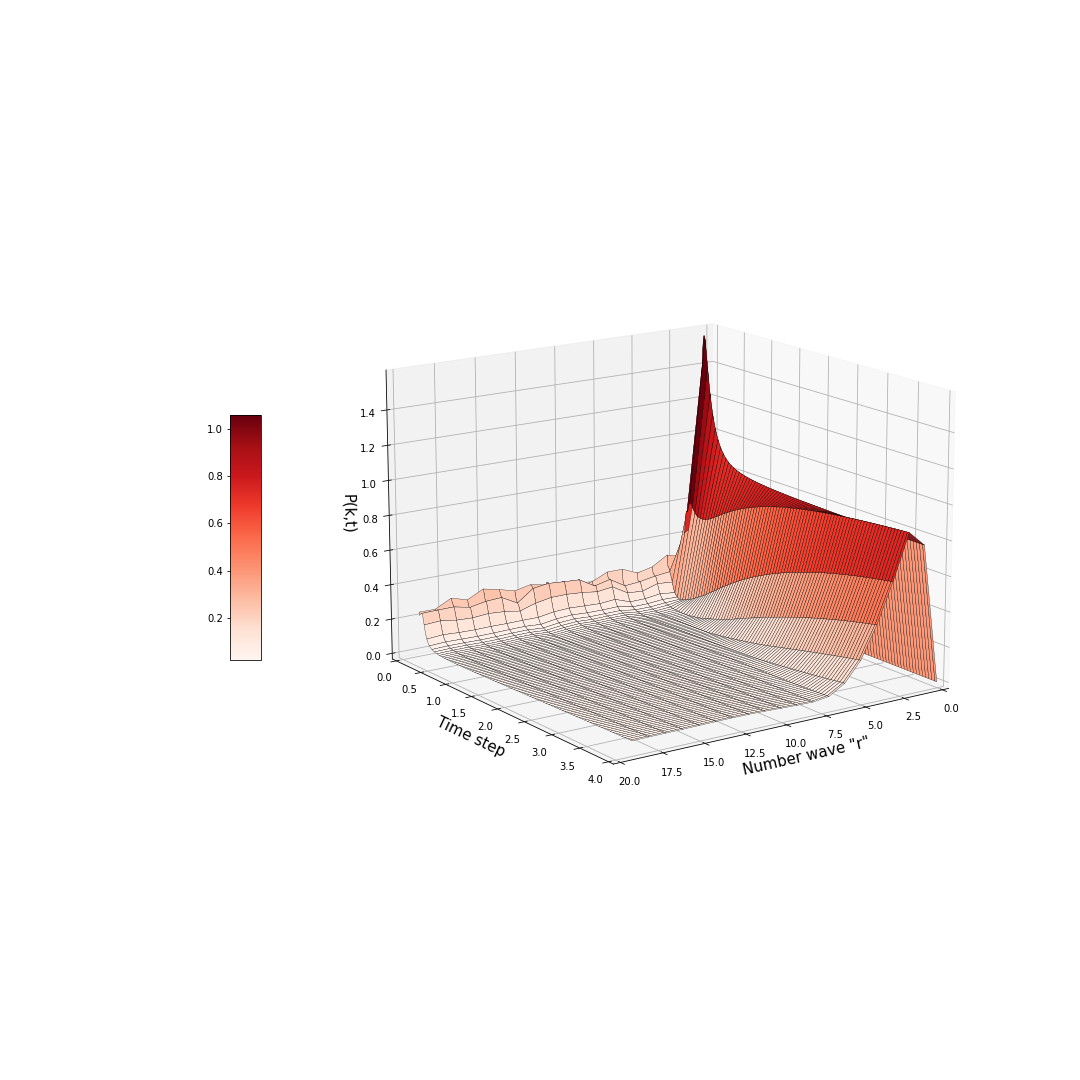
\includegraphics[width=0.7\textwidth]{images/correlations_3D_cc.png}
    \caption{}
\end{figure}

\begin{figure}[htbp]
    \centering
    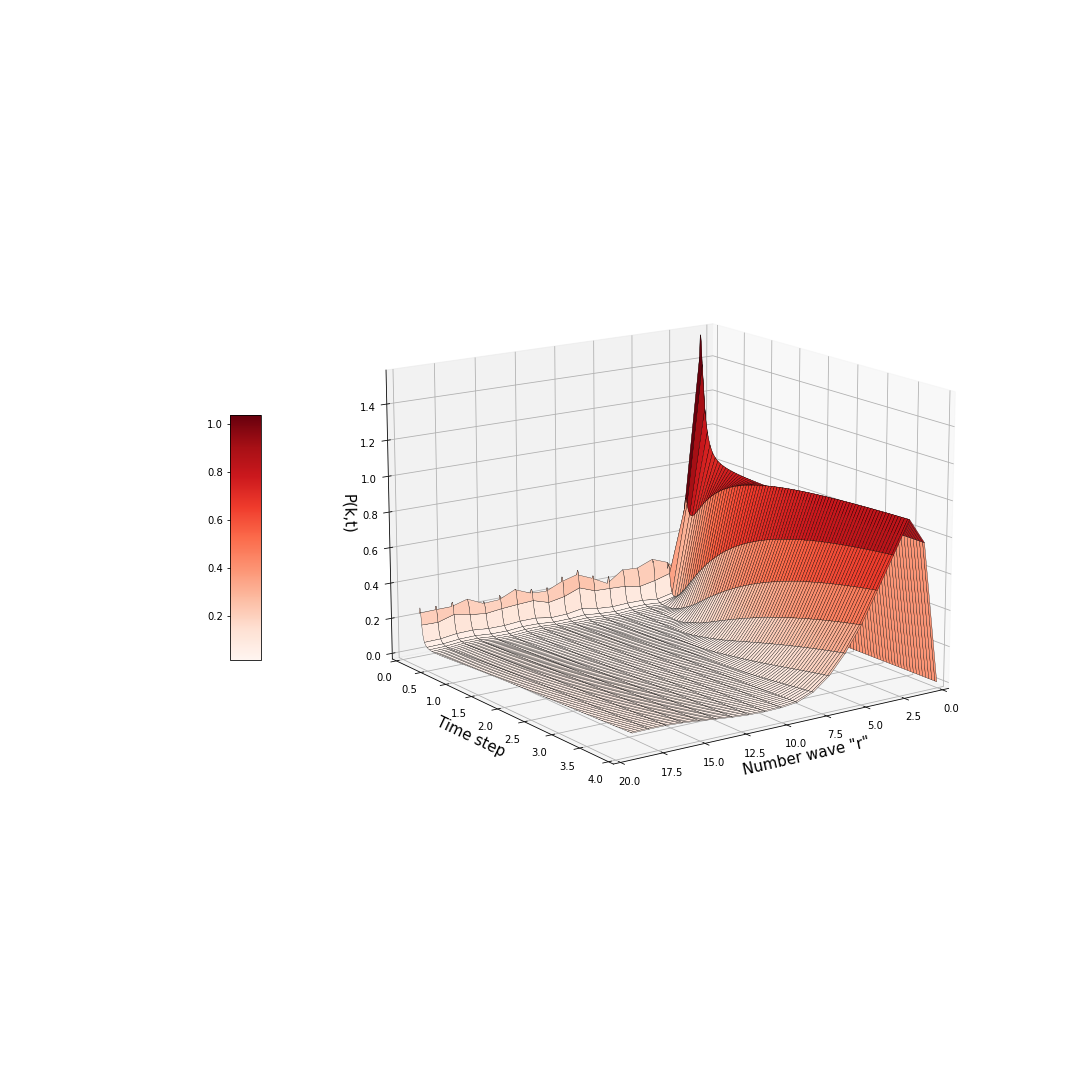
\includegraphics[width=0.7\textwidth]{images/correlations_3D_ss.png}
    \caption{}
\end{figure}


\begin{figure}[htbp]
    \centering
    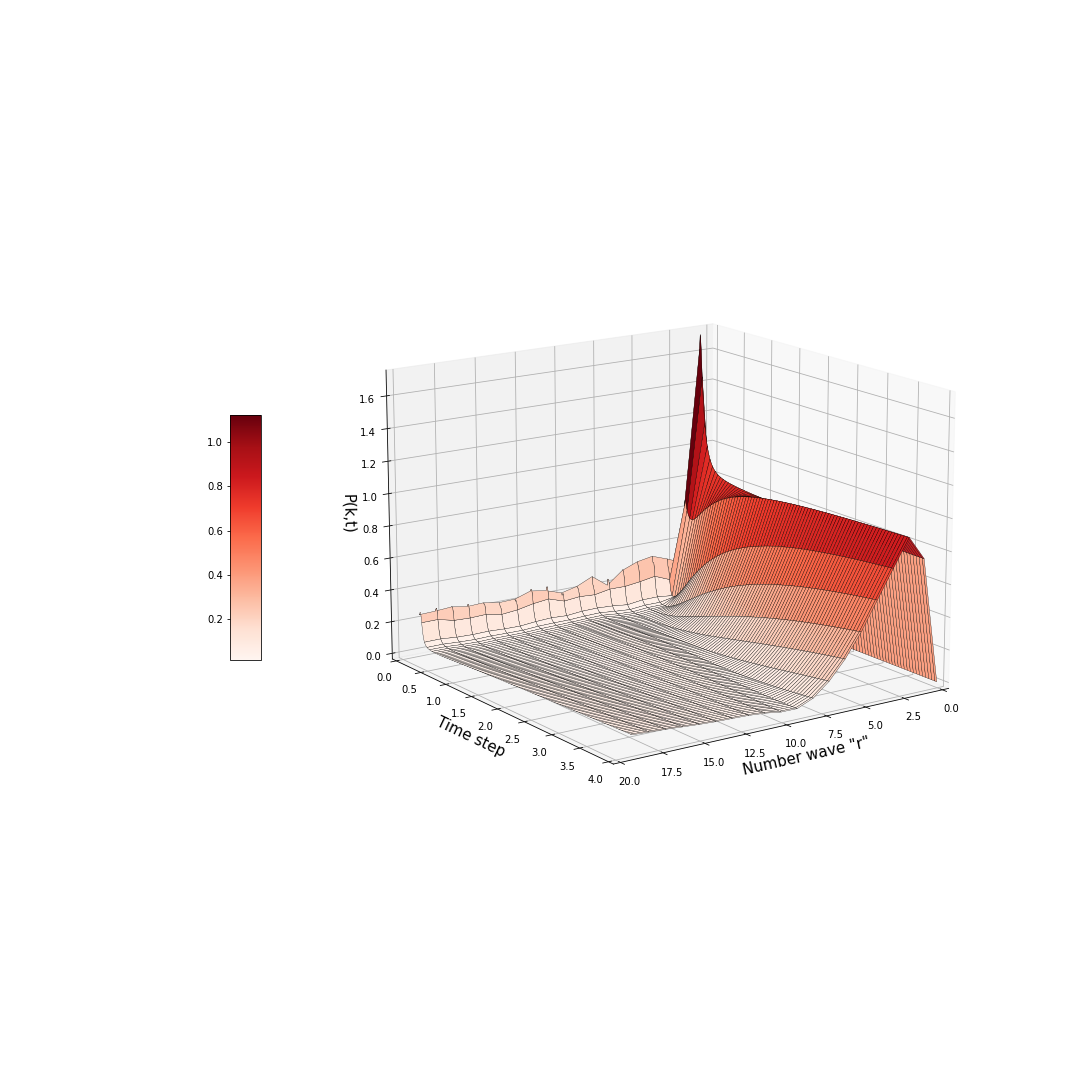
\includegraphics[width=0.7\textwidth]{images/correlations_3D_ii.png}
    \caption{}
\end{figure}



\subsubsection{Correlación Cruzada (correlaciones cs, ci, si)}

La correlación cruzada entre diferentes tipos de células te indica cómo se relacionan espacialmente. Por ejemplo, una alta correlación cruzada entre c y i podría sugerir que las células inmunitarias tienden a agruparse alrededor de las células cancerígenas.

\begin{itemize}
    \item cs, sc: Estas son las correlaciones cruzadas entre células cancerosas y sanas. Analizar estos términos puede darnos información sobre cómo las células cancerosas influyen en la distribución de las células sanas o viceversa. Una alta correlación positiva podría indicar que las células sanas y las células cancerosas tienden a coexistir en las mismas regiones, mientras que una correlación negativa podría sugerir que las células cancerosas desplazan a las células sanas.
    \item ci, ic: Estas correlaciones cruzadas entre células cancerosas e inmunitarias pueden revelar la efectividad de la respuesta inmunitaria contra las células cancerosas. Una correlación positiva alta podría sugerir que las células inmunitarias están respondiendo bien a la presencia de células cancerosas, mientras que una correlación negativa podría indicar que las células cancerosas están evadiendo la respuesta inmunitaria.
    \item si, is: Estas correlaciones cruzadas entre células sanas e inmunitarias pueden ofrecer informacion sobre la protección que las células inmunitarias brindan a las células sanas o sobre cómo estas dos poblaciones celulares interactúan en presencia de una enfermedad.
\end{itemize}


\begin{figure}[htbp]
    \centering
    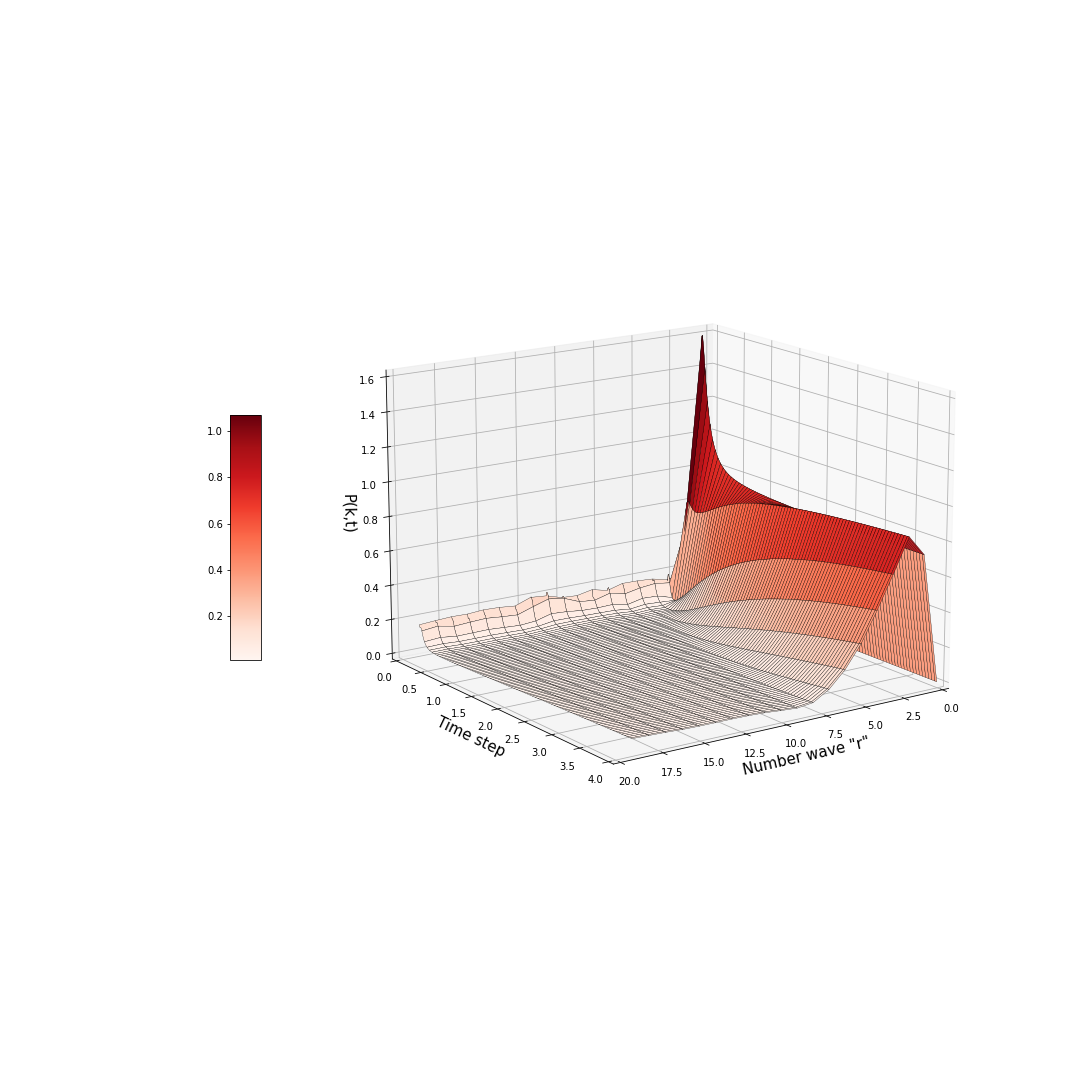
\includegraphics[width=0.7\textwidth]{images/correlations_3D_ci.png}
    \caption{Correlación c-i}
\end{figure}

\begin{figure}[htbp]
    \centering
    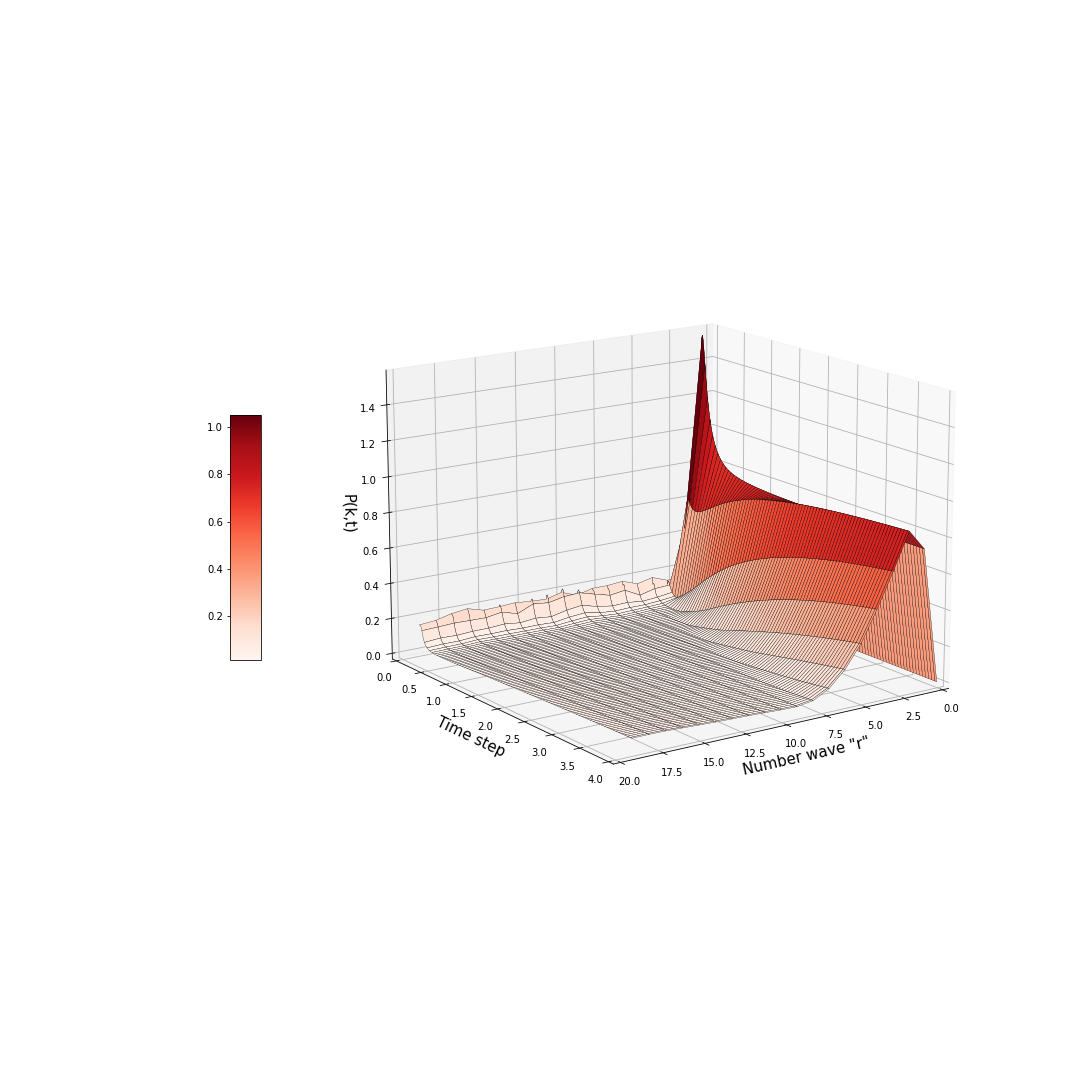
\includegraphics[width=0.7\textwidth]{images/correlations_3D_cs.png}
    \caption{Correlación c-s}
\end{figure}


\begin{figure}[htbp]
    \centering
    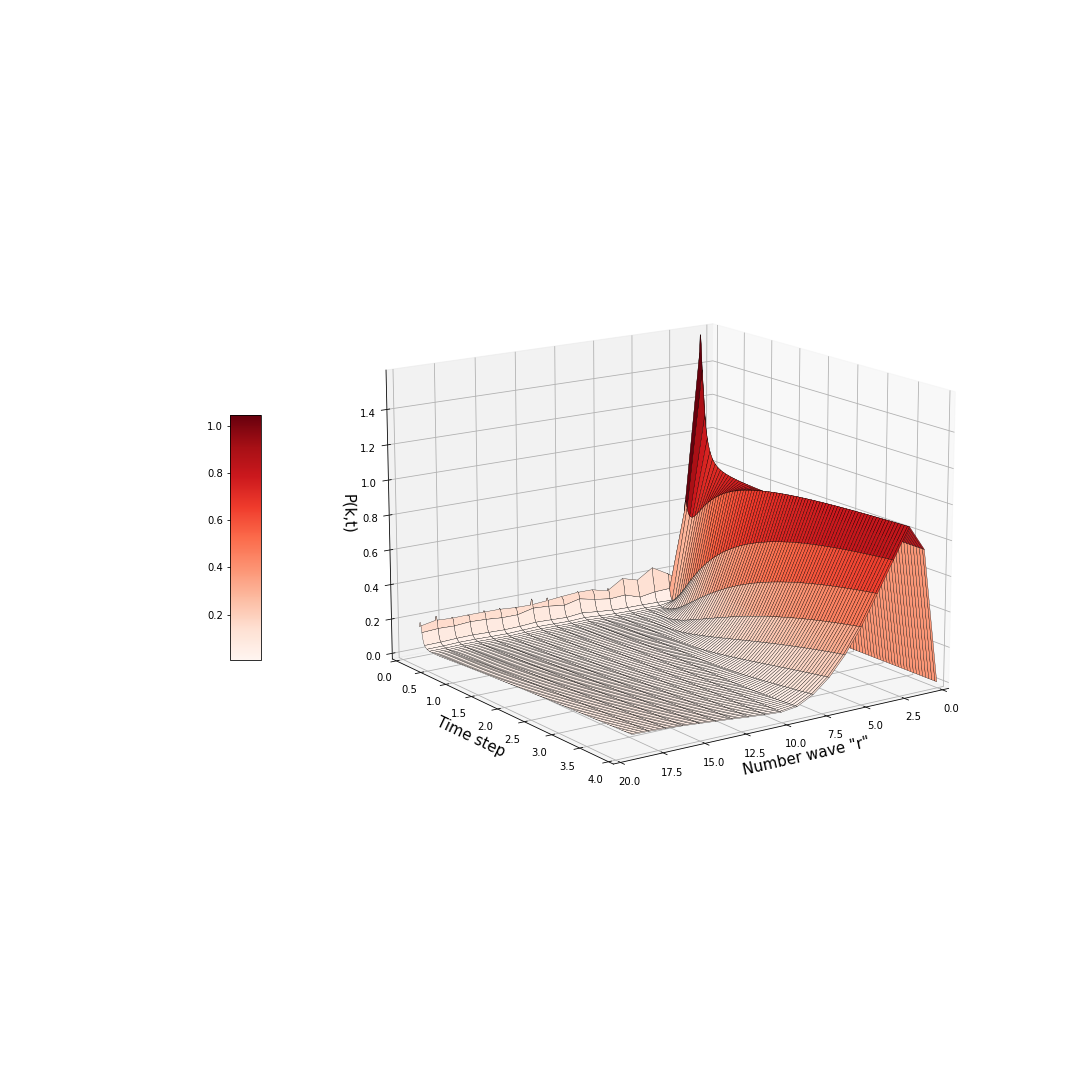
\includegraphics[width=0.7\textwidth]{images/correlations_3D_si.png}
    \caption{Correlación s-i}
\end{figure}



\textbf{Evolución de los campos inicialmente aleatorio pero con cancer concentrado en dos circunferencias de radio r} $0.7 < s < 0.9$ e $0.5 < i < 0.7$

\begin{itemize}
    \item Coordenadas donde el cáncer se origina: centers = [(5, 5), (15, 15)] 
    \item  radio = 1.0  
    \item Densidad fuera de los radios 0 
    \item Densidad dentro de los radios 10 por ciento  
\end{itemize}

\begin{figure}[htbp]
    \centering
    \includegraphics[width=1\textwidth, height=0.2\textheight]{images/fields_ci.png}
    \caption{}
    \label{fig:imagen}
\end{figure}

Este es un enlace al \href{https://drive.google.com/file/d/1Hl6HBr52QO_7C0TiIAbX3hWmhV7qsdj5/view?usp=sharing}{video de la evolución de los campos}.


\textbf{Promedio Polar} 

Este es un enlace al \href{https://drive.google.com/file/d/1wWUlXln6fIPdRKu395ER4sc2wQxrvNeg/view?usp=sharing}{Promedio c}, \href{https://drive.google.com/file/d/18-IVr3RBkPF6Sv-aQMYDcZRIQnAGa0_r/view?usp=sharing}{Promedio s} y \href{https://drive.google.com/file/d/1A0mJWxUnSsrAZmOuSexXsXKUz1pK-PkT/view?usp=sharing}{Promedio i}.
\\



\textbf{Autocorrelación Espacial (correlaciones cc, ss, ii)} \\

Este es un enlace las imagenes para \href{https://drive.google.com/file/d/1SKs6iYmqRfT2GZQ8uLqQVi3mwWwliuSi/view?usp=sharing}{autocorrelacion cc}, \href{https://drive.google.com/file/d/1SFWy_DRovIJkZfi-hlySh90VjTyjFTi2/view?usp=sharing}{autocorrelacion ss} e \href{https://drive.google.com/file/d/1e8Ux9X606QRTh7phvR9jggGsIyz37SiY/view?usp=sharing}{autocorrelacion ii} .



\textbf{Correlación Cruzada (correlaciones cs, ci, si)}\\

Este es un enlace las imagenes para \href{https://drive.google.com/file/d/1HQiLCoq0TXW7r0nOZmEUQbCo2mnua54I/view?usp=sharing}{correlacion cs}, \href{https://drive.google.com/file/d/1HbKgHtY2npXeVr5coQWs0DDWxdcN9sAi/view?usp=sharing}{correlacion ci} y \href{https://drive.google.com/file/d/1h3LXM1CiXaje-c24C6aUY6VlMhE6VyAb/view?usp=sharing}{correlacion si} .

\end{document}